\documentclass{beamer}

\usepackage{amssymb}
\usepackage{amsmath}
\usepackage{amsthm}
\usepackage{amsfonts}

\usepackage{multicol}

\usepackage{graphicx}
\graphicspath{ {./src} }

\usepackage{tikz}

\usepackage{pgfplots}
\pgfplotsset{compat = newest}

\usepackage{verbatim}
\usetikzlibrary{arrows,shapes}

% for cross reference
% \usepackage{hyperref}

% for fixed length of cell of tables
% \usepackage{tabularx}
% \usepackage{longtable}

\AtBeginSection[]
{
  \begin{frame}
    \frametitle{Table of Contents}
    \tableofcontents[currentsection]
  \end{frame}
}


\title{Communicate Without Errors}
\author{Zifan Hua}

\begin{document}

      \frame{\titlepage}

      \begin{frame}
            \frametitle[TOC]{Table Of Contents}
            \tableofcontents
      \end{frame}

      \section{Introduction}

      \begin{frame}
            \frametitle{Introduction}
            \begin{itemize}
                  \item Channel Capacity
                  \item Zero Error Rate
                  \item Shannon Capacity
                  \item $C_{n}$
                  \item $\sqrt{5} \le \Theta(C_{5}) \le 5/2$
                  \item $\Theta(G) = \sqrt{5}$ by Lovász László
            \end{itemize}
      \end{frame}

      \section{Some Definitions}

            \subsection{Channel}

                  \begin{frame}
                        \frametitle{Channel}
                        \begin{definition}[channel]
                              A channel has a sender and a receiver.
                              \pause


                              A message is a finite sequence of characters.
                              The sender sends a message to the receiver.
                              \begin{figure}[h!]
                                    \tikzstyle{vertex}=[fill=black!25,minimum size=20pt,inner sep=0pt]
                                    \tikzstyle{message}=[inner sep=0pt]
                                    \tikzstyle{edge} = [draw,thick,-]
                                    \tikzstyle{weight} = [font=\small]
                                    \begin{tikzpicture}[scale=1, auto,swap]
                                          % Draw a 7,11 network
                                          % First we draw the vertices
                                          \foreach \pos/\name in {{(0,0)/sender}, {(3,0)/receiver}}
                                                \node[vertex] (\name) at \pos {$\name$};
                                          \foreach \pos/\name in {{(0,1)/abcde}, {(3,1)/acbde}}
                                                \node[message] (\name) at \pos {$\name$};
                                          % Connect vertices with edges and draw weights
                                          \foreach \source/ \dest in {sender/receiver}
                                          \path[edge] (\source) -- node[weight]{} (\dest);
                                    \end{tikzpicture}
                              \end{figure}
                              \pause
                              
                              The receiver receives message and decode it.
                              \pause

                              However, in the procedure of send and receive, the channel may introduce some errors. For instance, here, character $b$ is decoded into $c$. 
                        \end{definition}
                  \end{frame}

                  \begin{frame}
                        \frametitle{Channel}
                        \begin{definition}[confusable]
                              Given two characters $a$, $b$. If $a$ and $b$ have chance to be decoded into a same character say $c$, we say $a$ and $b$ are confusable.

                              For a two messages of length $n$, say $a_{1}a_{2}\dots a_{n}$, $b_{1}b_{2}\dots b_{n}$ is confusable if and only if $a_{i}$ and $b_{i}$ are confusable for every $i$.
                        \end{definition}
                        \pause
                        \begin{definition}[rate of channel]
                              The rate of channel actually represent how many distinct character can be send per unit time.

                              Given a channel that could send $r$ distinct characters per unit time. And send message with length $n$, so the number of distinct messages the channel can send is $r^{n}$.

                              \pause

                              Conversely, given a channel that could send $m$ distinct messages with length $n$.
                              And could be able to send only one character per unit time.
                              The rate of channel is $\sqrt[n]{m}$.

                              Here, we do not care about how much characters. We only care about the number of all messages we can send.
                              
                        \end{definition}
                  \end{frame}

                  \begin{frame}
                        \frametitle{Channel}
                        \begin{definition}[zero error rate]
                              Given a channel which could transfer messages of length $n$.

                              We want to find the maximum set of messages $M$ that no two of them is confusable.

                              \begin{equation}
                                    \text{zero error rate} = \max_{M} \sqrt[n]{|M|}
                              \end{equation}
                        \end{definition}
                  \end{frame}

                  \begin{frame}
                        \frametitle{Channel}
                        If given a set of characters $S$, and some of the characters could be confusable.

                        We want to find
                        \begin{equation}
                              \sup_{n} \left\{
                                    \text{zero error rate of channel with length $n$ and $S$ as characters}
                              \right\}
                        \end{equation}

                        And we call this the shannon Capacity and denoted by $\Theta(S)$.

                        Clearly, shannon Capacity is actually a function of the set of characters. So, we want a more abstract way to represent the characters.
                  \end{frame}

            \subsection{Graph Representation of Characters}

                  \begin{frame}
                        \frametitle{Graph Representation Of Characters}
                        \begin{definition}[graph] \label{def:graph}
                              A graph $ G $ is a set of vertices with a set of edges connecting pairs of vertices.

                              \begin{figure}[h!]
                                    \tikzstyle{vertex}=[circle,fill=black!25,minimum size=20pt,inner sep=0pt]
                                    \tikzstyle{edge} = [draw,thick,-]
                                    \tikzstyle{weight} = [font=\small]
                                    \begin{tikzpicture}[scale=1, auto,swap]
                                          % Draw a 7,11 network
                                          % First we draw the vertices
                                          \foreach \pos/\name in {{(0,2)/a}, {(2,1)/b}, {(4,1)/c},
                                                {(0,0)/d}, {(3,0)/e}, {(2,-1)/f}, {(4,-1)/g}}
                                                \node[vertex] (\name) at \pos {$\name$};
                                          % Connect vertices with edges and draw weights
                                          \foreach \source/ \dest in {b/a, c/b,d/a,d/b,
                                                e/b, e/c,e/d,
                                                f/d,f/e,
                                                g/e,g/f}
                                          \path[edge] (\source) -- node[weight]{} (\dest);
                                    \end{tikzpicture}
                                    \label{fig:graphDefinitionExample}
                                    \caption{An example of a graph.}
                              \end{figure}
                        \end{definition}
                  \end{frame}

                  \begin{frame}
                        \frametitle{Graph Representation Of Characters}
                        \begin{definition}\label{def:graphRepresetationOfChannel}
                              Given a channel that sending $\{1,2,\dots,n\}$ as characters. And some characters $i$ and $j$ could be confused with each other.

                              Then the graph representation of the characters is the graph with vertices $\{1,2,\dots,n\}$ and edges $(i,j)$ if and only if $i$ and $j$ could be confused with each other.
                        \end{definition}

                        Accordingly, there is the corresponding way that using graphs to represent a message zero error rate and Shannon Capacity.
                  \end{frame}

            \subsection{Product Graph}

                  \begin{frame}
                        \frametitle{Product Graph}
                        \begin{definition}[graph product]\label{def:graphProduct}
                              The product of two graphs can be considered as send a pair of characters $(x,y)$ as one message. So, we have a channel that send messages of length $2$.

                              \pause

                              Recall that before, $2$ messages is confusable means that they can be decoded into the same message, which means every characters the two channel use need to be confusable.

                              Given two graph $ G $ and $ H $. The graph product $ G \times H $ is the graph with vertices $ V(G \times H) = V(G) \times V(H) $ in which $ (x,y) $ is adjacent to $ (x',y') $ in $ G \times H $ if and only if $ x $ is adjacent to $ x' $ in $ G $ and $ y $ is adjacent to $ y' $ in $ H $.
                  
                              \pause

                              A graph $ G $ product itself for $ n $ times will always be denoted by $ G^n $.

                              Which means we could use $ G^n $ to represent messages of a channel with length $n$.
                        \end{definition}
                  \end{frame}

            \subsection{Alpha Function}

                  \begin{frame}
                        \frametitle{$\alpha(G)$}
                        \begin{definition}[$\alpha(G)$]\label{def:alpha}
                              The $\alpha(G)$ represent the maximum number of characters or message that could not be confused with each other in graph $G$.

                              If $G$ represent a set of messages, $\alpha(G)$ is just the zero error rate we have defined before.

                              \pause

                              Given a graph $ G $. Given a subgraph $ H $ of $ G $, such that every vertex of $ H $ is not connected in $ G $. Then $ \alpha(G) $ is the maximum number of vertices of $ H $.
                              \tikzstyle{vertex}=[circle,fill=black!25,minimum size=20pt,inner sep=0pt]
                              \tikzstyle{selected vertex}=[circle,fill=red!25,minimum size=20pt,inner sep=0pt]
                              \tikzstyle{edge} = [draw,thick,-]
                              \tikzstyle{weight} = [font=\small]
                              \begin{figure}[h!]
                                    \begin{tikzpicture}[scale=1, auto,swap]
                                          % Draw a 7,11 network
                                          % First we draw the vertices
                                          \foreach \pos/\name in {{(0,1)/a}, {(2,1)/b}, {(4,1)/c},
                                                {(0,0)/d}, {(3,0)/e}, {(2,-1)/f}, {(4,-1)/g}}
                                                \node[vertex] (\name) at \pos {$\name$};
                                          \foreach \pos/\name in {{(0,1)/a}, {(4,1)/c},
                                                {(2,-1)/f}}
                                                \node[selected vertex] (\name) at \pos {$\name$};
                                          % Connect vertices with edges and draw weights
                                          \foreach \source/ \dest in {b/a, c/b,d/a,d/b,
                                                e/b, e/c,e/d,
                                                f/d,f/e,
                                                g/e,g/f}
                                          \path[edge] (\source) -- node[weight]{} (\dest);
                                    \end{tikzpicture}
                                    \label{fig:alphaGExample}
                                    \caption{Example of $ \alpha(G) $. Here $ \alpha(G) = 3 $.}
                              \end{figure}
                        \end{definition}
                  \end{frame}

            \subsection{Shannon Capacity}

                  \begin{frame}
                        \frametitle{Shannon Capacity}
                        \begin{definition}[Shannon Capacity]\label{def:shannonCapacity}
                              Recall that Shannon Capacity is 
                              \begin{equation}
                                    \sup_{n} \left\{
                                          \text{zero error rate of channel with length $n$ and $S$ as characters}
                                    \right\}
                              \end{equation}

                              Use the graph $G$ to represent the set of characters, the Shannon capacity $ \Theta(G) $ is defined by
                              \begin{equation}
                                    \Theta(G) = \sup_{n} \sqrt[n]{\alpha(G^n)} 
                              \end{equation}

                        \end{definition}
                  \end{frame}

      \section{The Real Solution}

                  \begin{frame}
                        To get the final result, we still need some more tools.
                  \end{frame}

            \subsection{Lemma 1}

                  \begin{frame}
                        \frametitle{Properties of $\alpha(G)$}
                        \begin{lemma}
                              $\alpha(G)\alpha(H) \leq \alpha(G \times H)$
                        \end{lemma}
            
                        \pause
            
                        \begin{proof}
                              Given graph $ G $ and $ H $. Let $ G' $ and $ H' $ be subgraph of $ G $ and $ H $ such that no vertex of $ G' $ or $ H' $ is adjacent in $ G $ or $ H $, respectively. Then $ G' \times H' $ is a subgraph of $ G \times H $ such that no vertex of $ G' \times H' $ is adjacent in $ G \times H $.
                        \end{proof}
                  \end{frame}

            \subsection{Orthonormal Representation}

                  \begin{frame}
                        \frametitle{Orthonormal Representation}

                        Here we have the third way to defined a set of characters.

                        \begin{definition}[Orthonormal Representation]\label{def:orthonormalRepresentation}
                              Given a graph $ G $ with vertices $ 1,2,\dots,n $, the orthonormal representation of $ G $ is a set of unit vectors $ \{v_1, v_2, \dots, v_n\} $ such that $ v_i $ and $ v_j $ are orthogonal if and only if $ i $ and $ j $ are not adjacent in $ G $.
                        \end{definition}

                        \pause

                        This existence of the orthonormal representation can be proved by induction.

                  \end{frame}

            \subsection{Tensor Product}

                  \begin{frame}
                        \frametitle{Tensor Product}
                        \begin{definition}[tensor product]\label{def:tensorProduct}
                              Given two vectors $ v = \left(v_{1},\dots,v_{n}\right) $ and $ w = \left(w_{1},\dots,w_{n}\right) $, the tensor product $ v \circ w $ is defined by
                              \begin{equation}
                                    v \circ w = \left(
                                          v_{1}w_{1},\dots,v_{1}w_{n},
                                          v_{2}w_{1},\dots,v_{2}w_{n},
                                          \dots,
                                          v_{n}w_{1},\dots,v_{n}w_{n}
                                          \right)
                              \end{equation}
                        \end{definition}

                        \pause

                        \begin{lemma}
                              The inner product of tensor products can be computed by,
                              \begin{equation}
                                    \langle v \circ w, v' \circ w' \rangle = \langle v, v' \rangle \langle w, w' \rangle
                              \end{equation}
                        \end{lemma}

                  \end{frame}

                  \begin{frame}
                        This is the product of graph in the sense of orthonormal representation.

                        \frametitle{Product of Orthonormal Representation}
                        \begin{lemma}
                              Given a graph $ G $ with vertices $ 1,2,\dots,n $, and a graph $ H $ with vertices $ 1,2,\dots,m $. Then vectors $\{ v_{i}\circ w_{j} \}$ is an orthonormal representation of $ G \times H $.
                        \end{lemma}
                  \end{frame}

            \subsection{Theta Function}

                  \begin{frame}
                        \frametitle{Theta Function}
                        Given a graph $ G $, the $ \theta(G) $ is defined by
                        \begin{equation}
                              \theta(G) = \inf_{\{v_1, v_2, \dots, v_n\},c} \max_{i} \frac{1}{\left<c,v_{i}\right>^2}
                        \end{equation}
                        where $ \{v_1, v_2, \dots, v_n\} $ is an orthonormal representation of $ G $, and c is any unit vector does not orthogonal to $ v_i $.

                        \pause

                        \begin{lemma}
                              There always exist such an $c$ and orthonormal representation $ \{v_1, v_2, \dots, v_n\} $ such that
                              \begin{equation}
                                    \theta(G) = \max_{i} \frac{1}{\left<c,v_{i}\right>^2}
                              \end{equation}
                        \end{lemma}

                        This could be proved by proving the set of all possible cases of $ \{v_1, v_2, \dots, v_n,c \} $ is compact. And the function $ \max \frac{1}{\left<c,v_{i}\right>^2} $ is continuous.
                  \end{frame}

            \subsection{Lemma 2}

                  \begin{frame}
                        \frametitle{Theta Function}
                        \begin{lemma}
                              Given graph $ G $ and $ H $, then
                              \begin{equation}
                                    \theta(G \times H) \leq \theta(G) \theta(H)
                              \end{equation}
                        \end{lemma}

                        \pause

                        \begin{proof}
                              Let $ \{v_1, v_2, \dots, v_n\} $ and $ \{w_1, w_2, \dots, w_m\} $ be orthonormal representation of $ G $ and $ H $ and $ c_{v} $ and $ c_{w} $ such that
                              \begin{equation}
                                    \max \left\{ \frac{1}{\left<c_{v},v_{i}\right>^2} : i=1,2,\dots,n \right\} = \theta(G)
                              \end{equation} 
                              and 
                              \begin{equation}
                                    \max \left\{ \frac{1}{\left<c_{w},w_{i}\right>^2} : i=1,2,\dots,m \right\} = \theta(H)
                              \end{equation}
                        \end{proof}
                  \end{frame}

                  \begin{frame}
                        \begin{proof}
                              Then
                              \begin{eqnarray}
                                    \theta(G \times H) &\leq& 
                                    \max \left\{ \frac{1}{\left<c_{v} \circ c_{w},v_{i} \circ w_{j}\right>^2} \right\} \\
                                    &=& \max \left\{ \frac{1}{\left<c_{v},v_{i}\right>^2 \left<c_{w},w_{j}\right>^2} \right\} \\
                                    &=& \max \left\{ \frac{1}{\left<c_{v},v_{i}\right>^2} \right\} \max \left\{ \frac{1}{\left<c_{w},w_{j}\right>^2} \right\} \\
                                    &=& \theta(G) \theta(H) \\
                              \end{eqnarray}
                        \end{proof}
                  \end{frame}

            \subsection{Lemma 3}

                  \begin{frame}
                        This lemma relates the $\theta(G)$ and $\alpha(G)$.

                        \begin{lemma}
                              \begin{equation}
                                    \theta(G) \geq \alpha(G)
                              \end{equation}
                        \end{lemma}

                        \pause

                        \begin{proof}
                              Let $ \{1,2,\dots,k\} $ be the set of vertices of $ G $ such that every point is not adjacency in $ G $. And $ k = \alpha(G) $
                  
                              Let $ \{v_1, v_2, \dots, v_n\} $ be an orthonormal representation of $ G $ and $ c $ such that
                              \begin{equation}
                                    \max \left\{ \frac{1}{\left<c,v_{i}\right>^2} \right\} = \theta(G)
                              \end{equation}
                                    
                              Then
                              \begin{eqnarray}
                                    1 &=& c^{2}
                                    \geq \sum_{i=1}^{k} \left<c,v_{i}\right>^{2}
                                    \geq \frac{k}{\theta(G)}
                              \end{eqnarray}
                        \end{proof}
                  \end{frame}

            \subsection{Theorem 1}
                  
                  \begin{frame}
                        \begin{theorem}
                              Given a graph $ G $, then
                              \begin{equation}
                                    \theta(G) \geq \Theta(G)
                              \end{equation}
                        \end{theorem}

                        \pause

                        \begin{proof}
                              \begin{eqnarray}
                                    \Theta(G) &=& \lim_{n} \sqrt[n]{\alpha(G^{n})} \\
                                    &\leq& \lim_{n} \sqrt[n]{\theta(G^{n})} \\
                                    &\leq& \lim_{n} \sqrt[n]{\theta(G)^{n}} \\
                                    &=& \theta(G)
                              \end{eqnarray}
                        \end{proof}
                  \end{frame}

                  \begin{frame}
                        The final result we want to prove today,
                        \begin{equation}
                              \Theta(C_{5}) \le \theta(C_{5}) \le \sqrt{5}
                        \end{equation}
                  \end{frame}

            \subsection{Theorem 2}

                  \begin{frame}
                        \begin{theorem}
                              \begin{equation}
                                    \theta(C_{n}) \leq \sqrt{5}
                              \end{equation}
                        \end{theorem}
                  \end{frame}

                  \begin{frame}
                        \begin{proof}
                              Consider an umbrella that has a handle and $5$ ribs that all have unit length. And also its handle is a unit vector.
                  
                              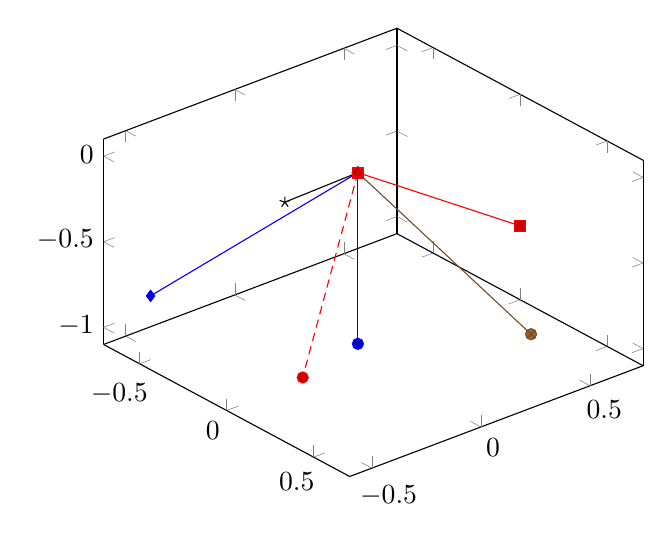
\begin{tikzpicture}
                   
                                    \begin{axis}[view = {50}{40}]
                                     
                                    \addplot3 coordinates 
                                    {
                                        (0,0,0)
                                        (0,0,-1)
                                    };
                  
                                    \addplot3 coordinates 
                                    {
                                        (0,0,0)
                                        (0,0.74349606,-0.66874031)
                                    };
                                     
                                    \addplot3 coordinates 
                                    {
                                        (0,0,0)
                                        (0.70710677,0.22975292,-0.66874031)
                                    };
                  
                                    \addplot3 coordinates 
                                    {
                                        (0,0,0)
                                        (-0.70710677,0.22975292,-0.66874031)
                                    };
                  
                  
                                    \addplot3 coordinates 
                                    {
                                        (0,0,0)
                                        (-0.43701602,-0.60150095,-0.66874031)
                                    };
                                    
                                    \addplot3 coordinates 
                                    {
                                        (0,0,0)
                                        (0.43701602,-0.60150095,-0.66874031)
                                    };
                  
                                    \end{axis}
                                     
                              \end{tikzpicture}

                        \end{proof}
                  \end{frame}

                  \begin{frame}
                        \begin{proof}
                              Here, angles between two consecutive ribs are same. 
                              
                              Let $v$ be a rib. And let $w$ be one of the rib that have the largest angle with $v$. Then, we let the angle between $v$ and $w$ be $ \pi/2 $.
                  
                              Then, the $5$ ribs of such an umbrella form an orthonormal representation of $C_{5}$.
                  
                              Let $d$ be the vector represent the handle, and $v_{1},v_{2},\dots,v_{5}$ be the $5$ ribs. And let $\gamma$ be the angle between the handle and any rib.
                  
                              So, by some calculation, we get
                              \begin{eqnarray}
                                    \theta(C_{5}) &\le& \max \frac{1}{<d,v_{i}>^{2}} \\
                                    &=& \left(
                                          \frac{1}{\cos(\gamma)}
                                    \right)^{2} \\
                                    &=& \sqrt{5}
                              \end{eqnarray}
                        \end{proof}
                  \end{frame}

      \section{Conclusion and Discussion}

            \begin{frame}
                  \frametitle{Conclusion}
                  \begin{itemize}
                        \item We have proved that $Theta(C_{5}) = \sqrt{5}$
                        \item We could actually proved that $\Theta(C_{n})$ is equal to $ n\frac{\cos(\pi/n)}{1+\cos(\pi/n)} $.
                  \end{itemize}
            \end{frame}

            \begin{frame}
                  \frametitle{Open Questions}
                  \begin{itemize}
                        \item Although $\Theta(C_{n})$ is equal to $ n\frac{\cos(\pi/n)}{1+\cos(\pi/n)} $, but we still don't know the exact value of $\Theta(C_{n})$. Even for $n=7$
                        \item Is there any good lower bound for $\Theta(C_{n})$?
                        \item Is there any patterns for $n$ such that $\Theta(c_{n})$ is hard to compute?
                  \end{itemize}
            \end{frame}

            \begin{frame}
                  \frametitle{Discussion}

                  In the real world cases, we always have some kind of relay between the sender and receiver. So the new channel is kind of composite of two channel. Can we compute Shannon Capacity these channels independently and then combine them together to get the Shannon Capacity of the new Channel?
            \end{frame}

      \section{Reference}

            \begin{frame}
                  \frametitle{Reference}
                  \begin{itemize}
                        \item \href{https://ieeexplore.ieee.org/stamp/stamp.jsp?arnumber=1055985}{On the Shannon Capacity of a Graph} by Laszlo Lovasz
                        \item \href{https://ieeexplore.ieee.org/stamp/stamp.jsp?tp=&arnumber=1056798}{The zero error capacity of a noisy channel} by Claude Shannon
                  \end{itemize}
            \end{frame}

\end{document}